%\documentclass[doublecol]{epl2} 
% or \documentclass[page-classic]{epl2} for one column style

% \usepackage{amsfonts}
% \usepackage{graphicx}
% \usepackage{url}
% \usepackage{float}
% \usepackage{latexsym}
% \usepackage{amsmath,amssymb}
% \usepackage{dcolumn}
% \usepackage{epsfig}
% \usepackage{textcomp}
% \usepackage{mathtools}
% \usepackage{multirow}
% \usepackage{algorithm}
% \usepackage{algorithmic}
% \usepackage{soul}
% \usepackage{color}
% \usepackage{amsmath}
% \usepackage{adjustbox}
%\newcommand{\todo}[1]{\textcolor{red}{TODO: #1}}

\setcounter{MaxMatrixCols}{10}
%TCIDATA{OutputFilter=Latex.dll}
%TCIDATA{Version=5.00.0.2606}
%TCIDATA{<META NAME="SaveForMode" CONTENT="1">}
%TCIDATA{BibliographyScheme=BibTeX}
%TCIDATA{LastRevised=Sunday, February 28, 2016 13:36:09}
%TCIDATA{<META NAME="GraphicsSave" CONTENT="32">}
%TCIDATA{Language=American English}

\newtheorem{theorem}{Theorem}
\newtheorem{acknowledgement}[theorem]{Acknowledgement}
\newtheorem{axiom}[theorem]{Axiom}
\newtheorem{claim}[theorem]{Claim}
\newtheorem{conclusion}[theorem]{Conclusion}
\newtheorem{condition}[theorem]{Condition}
\newtheorem{conjecture}[theorem]{Conjecture}
\newtheorem{corollary}[theorem]{Corollary}
\newtheorem{criterion}[theorem]{Criterion}
\newtheorem{definition}[theorem]{Definition}
\newtheorem{example}[theorem]{Example}
\newtheorem{exercise}[theorem]{Exercise}
\newtheorem{lemma}[theorem]{Lemma}
\newtheorem{notation}[theorem]{Notation}
\newtheorem{problem}[theorem]{Problem}
\newtheorem{proposition}[theorem]{Proposition}
\newtheorem{remark}[theorem]{Remark}
\newtheorem{solution}[theorem]{Solution}
\newtheorem{summary}[theorem]{Summary}
\def\dint{\mathop{\displaystyle \int}}
\def\diint{\mathop{\displaystyle \iint }}
\def\diiint{\mathop{\displaystyle \iiint }}
\def\diiiint{\mathop{\displaystyle \iiiint }}
\def\didotsint{\mathop{\displaystyle \idotsint }}
\def\doint{\mathop{\displaystyle \oint}}
\def\dsum{\mathop{\displaystyle \sum }}
\def\dprod{\mathop{\displaystyle \prod }}
\def\dbigcap{\mathop{\displaystyle \bigcap }}
\def\dbigwedge{\mathop{\displaystyle \bigwedge }}
\def\dbigoplus{\mathop{\displaystyle \bigoplus }}
\def\dbigodot{\mathop{\displaystyle \bigodot }}
\def\dbigsqcup{\mathop{\displaystyle \bigsqcup }}
\def\dcoprod{\mathop{\displaystyle \coprod }}
\def\dbigcup{\mathop{\displaystyle \bigcup }}
\def\dbigvee{\mathop{\displaystyle \bigvee }}
\def\dbigotimes{\mathop{\displaystyle \bigotimes }}
\def\dbiguplus{\mathop{\displaystyle \biguplus }}
\def\BF#1{{\bf {#1}}}
\def\NEG#1{\leavevmode\hbox{\rlap{\thinspace/}{$#1$}}}



% \title{Threshold-based epidemic dynamics in systems with memory}
% \shorttitle{Threshold-based epidemic} %Insert here a short version of the title if it exceeds 70 characters
% 
% \author{Marcin Bodych\inst{2}, Niloy Ganguly\inst{1}, Tyll Krueger\inst{2}, Animesh Mukherjee\inst{1}, Rainer Siegmund-Schultze\inst{3} \and Sandipan Sikdar\inst{1}}
% \shortauthor{M. Bodych \etal}
% 
% \institute{                    
%   \inst{1} Indian Institute of Technology Kharagpur - Kharagpur, India - 721302\\
%   \inst{2} Wroclaw University of Technology - 27 50-370 Wrocław, Poland \\
%   \inst{3} Technical University Berlin - 10623 Berlin, Germany
% }
% \pacs{89.75.Hc}{First pacs description}
% \pacs{89.75.Fb}{Second pacs description}
%\pacs{nn.mm.xx}{Third pacs description}


% \abstract{
% In this article we analyze an epidemic dynamics model (SI) where 
% we assume that there are $k$ susceptible states, that is a node would require multiple ($k$) contacts before it gets infected. 
% In specific, we provide a theoretical framework for studying diffusion rate in 
% complete graphs and $d$-regular trees with extensions to dense random graphs. We observe that irrespective of the topology, the diffusion process could be 
% divided into two distinct phases: (i) the {\em initial} phase, where the diffusion process is slow, followed by (ii) {\em residual} phase where the diffusion rate 
% increases manifold. In fact, the initial phase acts as an indicator for the total diffusion time in dense graphs. 
% The most remarkable lesson from this investigation is that such a diffusion process {\em could be controlled and even contained if acted upon within its initial phase}.}
% 
% 
% \begin{document}
% 
% \maketitle


% \section{Section title}
% Insert here the text.
% See fig.~\ref{fig.1}, table~\ref{tab.1} and eq.~(\ref{eq.1}).
% See also~\cite{b.a,b.b}.
% \begin{equation}
% \label{eq.1}
% 0\neq1
% \end{equation}
% 
% 
% \begin{figure}
% \onefigure{epl-template.eps}
% \caption{Figure caption.}
% \label{fig.1}
% \end{figure}
% 
% 
% \begin{table}
% \caption{Table caption.}
% \label{tab.1}
% \begin{center}
% \begin{tabular}{lcr}
% first  & table & row\\
% second & table & row
% \end{tabular}
% \end{center}
% \end{table}
\chapter{Diffusion in temporal networks}
Previous two chapters dealt with analyzing structural properties of temporal networks. This chapter is devoted towards the functional aspect of time-varying networks.  
In specific, we are interested in studying diffusion dynamics in these networks. 
This chapter is divided into two parts. To start with we propose a threshold based diffusion model and systematically analyze the diffusion rate for different underlying 
graph topologies. We then leverage these results to obtain a message broadcast algorithm in dynamic networks. 


\noindent
\section{Introduction}
Information diffusion is one of the most common phenomena that occurs on a
network and the most elementary model of this process is SI
(Susceptible-Infected)~\cite{anderson1992infectious} and its different variations~\cite{watts2002simple,dodds2004universal,pnas1,pnas2,tang2009epidemic,son2012percolation}.
Epidemic/adoption models have recently found a renewed interest with the formulation of temporal networks and 
realization that most of the real-world networks are temporal in nature (network structure changes with time). 
\if{0}
For example,  Takaguchi et. al. in~\cite{takaguchi2013bursty} presents a model whereby adoption behavior 
of a node is driven by the number of recent contacts with already adopted individual. 
Through simulations on real-world temporal networks the authors further show that burstiness~\cite{karsai2011small} 
affects spreading rate. Similar empirical study was also performed by Karimi et. al. in~\cite{karimi2013threshold}. A further modification to the 
model has been proposed by Backlund et. al. in~\cite{backlund2014effects} which considers that adoption is driven by the number of contacts
with different adopted neighbors within a chosen time instead of a particular neighbor multiple times. Further, information diffusion on temporal 
networks, more specifically prevalence, have also been studied in \cite{rocha2013bursts}. 
Several other results on the study of 
epidemics in temporal networks are listed in~\cite{masuda2013predicting} and on epidemic thresholds in~\cite{prl1,van2012epidemic,zhang2014susceptible}.
This type of history-dependent thresholding spreading pattern is largely observed in spread of bacterial diseases such as tuberculosis and 
dysentery \cite{joh2009dynamics} and 
also in peer-to-peer \cite{sanghavi2007gossiping} and Bittorrent systems \cite{qiu2004modeling}. In \cite{romero2011differences} the authors show that people 
accept ideas/news after repeated exposure.
\fi

The fundamental difference between static and temporal epidemic (SI) models is that in temporal models every agent  within a population is {\em not equally susceptible} to a disease or equally amenable to a rumor
 - the one which has been exposed more number of times (in recent past) are more amenable. This difference however is not well formulated and hence not well modeled - the primary contribution of this work 
is to succinctly define the problem in  terms of a simple model and then theoretically calculate the rate of spread of the epidemics. 
%Albeit a deep literature exists on the study of epidemics in temporal networks, they are mostly simulation based and to the best of our knowledge, a theoretical foundation on the topic is still wanting. 
We consider a spreading model in the lines of~\cite{takaguchi2013bursty} where each susceptible node needs to communicate with the 
infected nodes {\em multiple times} to contract infection. More importantly, unlike memoryless systems, we assume that each node comprises a memory which 
keeps track of the number of contacts it makes with infected ones. Note that in our system memory is a property which allows each node to remember the number 
of contacts it has already made with the infected ones. While Karimi et. al. studied the effect of burstiness in the diffusion process, we 
are more interested in estimating both empirically and analytically the diffusion time and rate.
Note that this model is completely different from  threshold models~\cite{granovetter1978threshold,sur1} where a node
 gets infected when majority of its neighbors are infected or probabilistic SI-models where an infected node,  on coming in contact, 
infects a susceptible node with a probability $p$,  as those are memoryless systems and the transition depends only on the activity of present time step. 
Our diffusion model also differs from the Neighborhood Exchange (NE) model proposed in \cite{volz2007susceptible}. NE assumes at any given time, an individual
will be in contact with an individual-specific number of neighbors with whom disease transmission is possible while our model considers that a node can be in contact with 
only a single individual. Also NE does not consider the fact that multiple contacts are required to contract infection.

The analytical results are obtained 
considering simple yet important topologies like the complete graph and the infinite $d$-regular trees which accounts for two extreme variants of network topology in terms of edge 
density. 
We demonstrate that the total diffusion time required for complemete graph topology (with $n$ nodes) scales as $n^{\frac{k-1}{k}}$ where $k>1$ is the number 
of contacts required to infect a susceptible individual. 
This is in sharp contrast to the case with $k$ = $1$, where it has been shown that diffusion time 
scales as $\log{(n)}$ ~\cite{rumarSreadingPushPull,rumourSpreading_evolvingGraph_PushPull}.
Another important inference we draw from the theoretical analysis is that irrespective of the topology the diffusion process could be divided into two phases: (i) an initial phase where the diffusion rate is very slow and 
(ii) a residual phase where the diffusion becomes very fast.
This inference is also a crucial contribution of this work which can help in containing 
the spread of infectious diseases with minimum overhead if acted upon in the initial phase which we further prove through a detailed empirical study.


\medskip

\input{./texfiles/Chapter_3/netsci/Infocom2015_introduction}
\noindent
\section{Diffusion model}
\label{diffusion_model}
% \begin{figure*}
%  \centering
%  \includegraphics*[scale=0.35]{figs1/diffusion.eps}
%  \caption{\label{diff_mod} Diffusion model: A is infected while B, C, D are susceptible ($k=2$). At t=1 A communicates with C. At t=2 A communicates 
%  with D. At t=3 A again communicates with C. At this point C has communicated with an infected individual (A) twice. So C becomes infected and would remain so 
%  for the whole duration of the diffusion process.}
% \end{figure*}


% Here we describe the overall framework and information diffusion technique
% that we assume for the rest of our study. 
%We assume a network network topology $G = <V,E>$ where $V$ represent the set of nodes and $E$ represent a set of edges between the nodes.
 
\if{0}
Our framework essentially resembles the Susceptible-Infected (SI) epidemic spreading model where we assume
a node can be in one of the two states - (i) susceptible or (ii)
infected. Susceptible nodes are the ones which do not have the
information or are not infected but can get infected if they come in contact
with an infected node. Similarly, an infected node is one which
already have the information and at each discrete time step randomly
selects one of its neighbors and tries to infect it. Note that we use the terms 
information and infection interchangeably as they essentially denote the
same thing in the context of the current study. 
%Since the model is motivated from the idea that an individual requires persuasion
%from the adopters before she adopts an idea, we quantify persuasion by the
%number of contacts she makes with the adopters in the network.
%Infected nodes are the oneswith the information and are trying to spread it while susceptibles are the ones without the information and can only receive it from an infected node.
\fi
 \begin{figure}[htpb]
 %\vspace{-0.8cm}
  \centering
  \includegraphics[scale=0.37]{./texfiles/Chapter_3/epl/figs1/dynamics.pdf}
  %\includegraphics*[scale=0.28]{figs1/plot_var_k.eps}
 %\includegraphics*[scale=0.15]{figs/T1_vs_exp_T1_d_reg.eps}
 
%\hspace{5mm}(a)\hspace{75mm}(b) 
%\vspace{-2mm}
 \caption{\label{fig_dynamics}Proposed diffusion model for $k=2$.}
 %\vspace{-.5cm}
\end{figure}
 
 
 \begin{figure}[htpb]
 %\vspace{-.5cm}
  \centering
  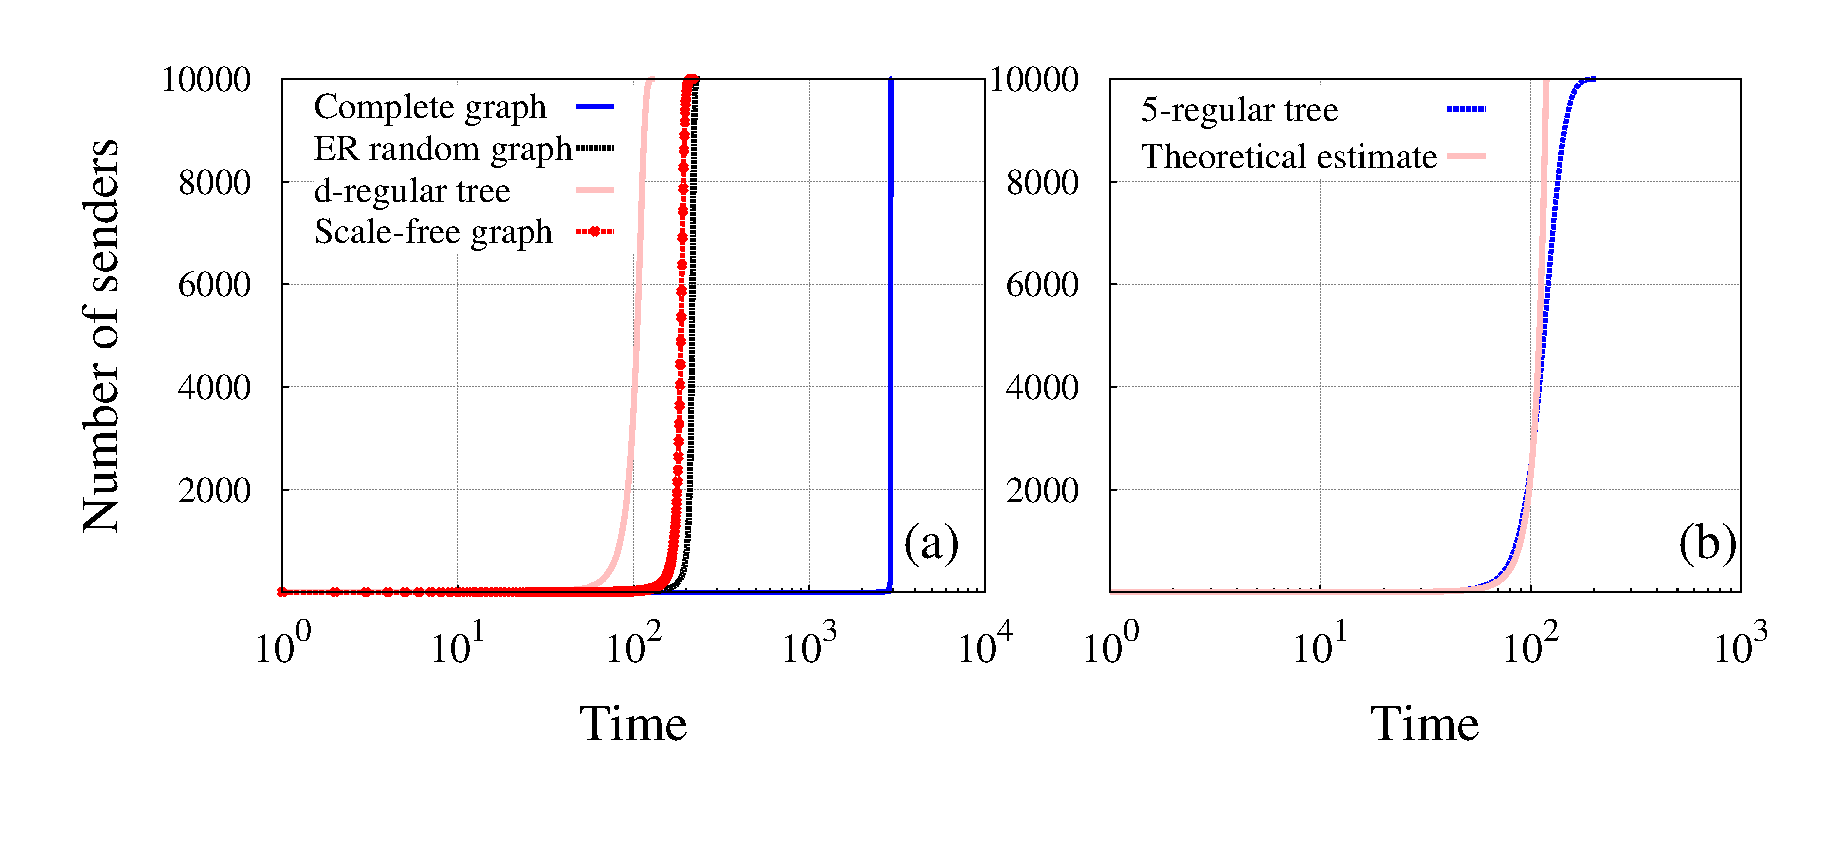
\includegraphics[scale=0.38]{./texfiles/Chapter_3/epl/figs1/plot_all.eps}
  %\includegraphics*[scale=0.28]{figs1/plot_var_k.eps}
 %\includegraphics*[scale=0.15]{figs/T1_vs_exp_T1_d_reg.eps}
 
%\hspace{5mm}(a)\hspace{75mm}(b) 
%\vspace{-4mm}
 \caption{\label{fig1} (a) The number of senders versus time steps for different network topologies (For ER random graph $p$ is $0.005$, for $d$-regular graph $d=5$ and for BA scale-free graph $m$ i.e., number of edges to attach from a new node to existing nodes is $5$) and 
 (b) The theoretical estimate and the simulated result for $d-$regular trees. The theoretical eastimate is obtained from equation 17.}
 \vspace{.5cm}
\end{figure}
 
% \todo{In figure~\ref{fig1} caption, add the vlaue of $p$ for ER graph and $\lambda$ for the scale-free graphs.}
 
Formally, we consider a network topology $G$ = $(V,E)$ where $V$ represents the set of
nodes in the network and $E$ denotes the set of edges between any pair of nodes in $%
V $. We initially start with a single infected node in the system. We
further assume that for a susceptible node to get infected,  $k$ encounters
with infected nodes are required. To put it in a simple way we consider that
a message $M$ needs to be spread over a network and message $M$ consists of $%
k$  identical tokens. At each communication instance one token gets transmitted from an
infected node to the susceptible node. Therefore, number of tokens ($k$) in a
message corresponds to the number of contacts required for a susceptible
node to get infected. Note that for the rest of this chapter we will present
our diffusion model in terms of messages and tokens. 
%Since the infected nodes essentially pass on the tokens we term them as senders while the susceptible ones are the non-senders.  

We assume that at time $0$, there is only one sender (infected) node present in the
system and it acts as the {\em initiator} of the diffusion process. At each
discrete time step a sender node randomly selects one of
its neighbors and  there is a transfer of a token from the sender to the non-sender. A non-sender node becomes a sender only after it receives exactly $k$
tokens (refer to figure \ref{fig_dynamics}). 
The analytical
estimation of the diffusion time based on the underlying topology requires a
case-by-case examination.
We formulate both analytical and empirical results for two extreme variants (in terms of edge density) of networks (a) complete graphs (dense) and (b) infinite regular trees (sparse)
while for others we provide empirical
results with intuitive justifications.
%\todo{Can we have a small picture demonstrating the dynamics since this is a very novel concept? We can take a small network, $k=3$ and illustrate the spread in three time points -- $t=0$ where only one node is black (the initiator), some intermediate $t=t^{'}$ where we show the $k$ values for different nodes (none of which is yet $=3$) and then $t=t^{''}$ where the first sender is formed (one node has $k=3$). We have enough white spaces between figures which can be reduced to fit in this picture.}
\if{0}
%Note that this results in creation of a subgraph at each time step roughly resembling a temporal network. 
% Assuming such a diffusion model we study in detail the diffusion time (i.e.,
% the time from the start till the time when all the nodes in the network
% receive the information and the algorithm terminates) given an underlying
% network topology.
\fi
% \begin{figure}[htpb]
%   \centering
%   \includegraphics[scale=0.28]{figs1/plot_var_k.eps}
%   %\includegraphics*[scale=0.28]{figs1/plot_var_k.eps}
%  %\includegraphics*[scale=0.15]{figs/T1_vs_exp_T1_d_reg.eps}
%  
% %\hspace{5mm}(a)\hspace{75mm}(b) 
%  \caption{\label{fig_k} Number of nodes at each stage of infection versus time for complete graph \todo{write more detailed description}}
% \end{figure}


\if{0} 
% \subsection{Agent configuration and network setup}
% 
% We consider a network topology $G = < V,E >$ where each node in $V$ represents an agent of the network and any link in $E$ represents a contact 
% opportunity between a pair of nodes (agents) in the whole time span through which the network is active. So for any node (agent) $n_{i}$ in this network, its one hop 
% neighbors are the nodes (agents) which are within the connection proximity of $n_{i}$ and at each time step $n_{i}$ at random can connect to any one of them. 
% 
% 
% \subsection{Information configuration}
% 
% As we stated earlier, we consider that the information diffusion occurs in parts. 
% We consider that thdie whole information $\mathcal{M}$ is divided into a set of $m$ tokens, i.e., $|\mathcal{M}| = m$ and in 
% a contact opportunity a single token gets transmitted.
%  We can also extend it to knowledge diffusion or special cases of disease spreading where a susceptible node gets infected 
%  only after it meets infected individuals for specified number of times. In these cases the total number of tokens 
%  would refer to the number of times ($m$) a susceptible (novice) individual communicates with an infected (knowledgeable) individual 
%  before it itself gets infected (knowledgeable). It can further be interpreted as the number of times a node should be reminded of an 
%  information before it remembers and participates in the diffusion process. Note that throughout our analysis we will stick to the 
%  notion of information and tokens for simplicity. 
% 
% 
% \subsection{Information diffusion technique}
% 
% In this framework, transfer of a message during a contact refers to the transfer of one single token of the information. 
% Transfer of a token from $u_i$ to $v_j$ during a contact can take place only 
% when $u_i$ qualifies as a {\em sender} by having all the tokens of the information.
% We mainly consider the $push$ technique of information diffusion which is described below. 
% 
% 
%  \noindent \emph{Push technique:} 
%   \begin{itemize}
%  % \vspace{-3mm}
%    \item \emph{Step 1:} At any time step, $u_i$ (already a sender) establishes a communication link with $v_j$, 
%    from its neighborhood and finds an exclusive set of tokens that $u_i$ has but $v_j$ does not have in its buffer. 
%    \item \emph{Step 2:} If $u_i$ can find such a (non-empty) set, then it transfers only one token from this set to $v_j$. 
%   \end{itemize}
% 
% Next we describe the information diffusion technique which we call $Blind Push$ (B-P) in detail.
% An initiator node is the one which has the full information in the beginning. At each time step all the nodes 
% in the system having the full information communicate with a node in their proximity and try to $push$. 
% %If it is successful then a unit bandwidth is consumed otherwise it is counted as wastage. 
% At the end of each time step all the nodes which have received all the tokens qualify as sender in the next time step. The algorithm terminates 
% when all the nodes in the system have the full information.
% We consider two types of epidemic processes - a) Susceptible-Infected (SI) and b) Susceptible-Infected-Recovered (SIR). 
% Susceptible nodes are the ones having a subset ($S$) of all the tokens ($0\leq |S| < m$, partial information) and the infected nodes are the one with 
% all the tokens (full information). The recovered nodes are the ones, which after having received the full information and spreading it for some time 
% have moved out of the system and is no longer part of the network.
% The information diffusion technique is similar for both the process. 

% \begin{algorithm}
% \caption{Blind Push (B-P)}\label{bp}
% \begin{algorithmic}[1]
% %\Procedure{MyProcedure}{}
% \STATE $select \, initiator$
% \STATE $make \, it \, sender$
% %\BState \emph{top}:
% %\If {$i > \textit{stringlen}$} \Return false
% %\EndIf
% %\State $j \gets \textit{patlen}$
%  \WHILE {$( not \, all \, nodes \, in \, the \, network \, have \, the \, message )$}
%  \FOR {$(each \, node \, which \, is \, already \, a \, sender)$}
% \STATE $select \, a \, node \, from \, its \, proximity;$
% \STATE $perform \, Push$;
% \IF {$(Push \, unsuccessful)$}
% \STATE $wastage;$
% \ELSE 
% \STATE $unit \, bandwidth \, consumed;$
% %\State $i \gets i-1$.
% %\State \textbf{goto} \emph{loop}.
% %\State \textbf{close};
% \ENDIF
% \ENDFOR
% \STATE $modify \, the \, list \, of \, senders;$
% \STATE $increment \, time;$
% \ENDWHILE
% %\EndProcedure
% \end{algorithmic}
% \end{algorithm}

% \subsection{Metrics of interest}
% %\vspace{-2mm}
% We are interested in evaluating the spreading model in terms of the following metrics-
% \begin{itemize}
% %\vspace{-4mm}
%  \item \textbf{Diffusion time $T^*$} - this is the time from the point when the message source starts the diffusion process to the point when all the agents in the network have received the the total information. 
%  $E(T^*)$ denotes the expected diffusion time. In addition, we are also interested in the time $T_i$ which is the minimum time at which there are $i$ senders (except the source) in the network, and especially in $T_1$ since, as we shall see, that this is the prime determinant of the entire broadcast time. 
% %\todo{why are these lines needed - Finally, note that $T^*$ may not correspond to $T_{n-1}$, i.e., the time when there are $n-1$ senders (except the source) in the network because all $n-1$ agents need not become senders to spread the message.}  
%  \item \textbf{Diffusion threshold} - 
% \end{itemize}
% \subsection{Dynamic topology}
% %\vspace{-2mm}
% We performed our experiments on synthetic topologies like complete graph, regular tree, regular graph and random graph. 
% A topology specifies the potential neighborhood of a node 
% - a node at each time step connects randomly to one of these nodes. A complete graph 
% topology would indicate that the 
% node can connect to any other node in the network while for other sparser topology it would 
% connect only to a subset of them.

\medskip
\fi



\noindent
\section{On complete graph}
\label{res_complete}
\noindent For {\bf complete graph} we assume the
number of nodes in the system to be $n$. 
%The time elapsed before the first sender (apart from the initiator) is created is represented by $t_1$ and the total diffusion time is denoted by $T^*$. We denote the expected values of these quantities by $% \mathbb{E}(t_1)$ and $\mathbb{E}(T^*)$ respectively. 
To determine how the number of
senders in the system changes with time, we plot the number of senders
against time for complete graph in figure~\ref{chapter_5_fig1}. 
%We further show in ~\ref{fig_k} how the diffusion progresses by plotting the number of nodes at each stage of infection at every time step for complete graph topology which roughly resembles epidemic process on a heterogenous population.  %Note
%that we assume the $d$-regular tree to be truncated with all the nodes except the leaf
%nodes have degree $d$.
We observe that the diffusion is initially slow which is then followed by a ramp-up after which the diffusion rate becomes almost exponentially fast.
To better analyze the process we divide the process into two phases i) the initial phase and ii) the residual phase. 


\noindent{\bf Initial phase:}  In the spreading process we define the initial phase to be the time between the
initiation and the point at which the first sender is created. We
define this as $t_1$; we will show later that $\hat E(t_1)$ (expected value of $t_1$) is
indeed an indicator for $\hat E(T^*)$ ($T^*$ - 
total diffusion time) in case of a complete graph.

Note that analytically deriving  $\hat E(t_1)$ assuming a  discrete 
(i.e., for a node the delay between two successive contacts is $1$ unit) diffusion model becomes severely complex and hence we adopt a continuous 
variant of the model. In fact, the calculation of the $\Pr \{ t_{1}=t\}$ can be treated as an expected time of filling the first urn with $k$
balls in the experiment where we have initially $d$ empty urns (degree of the node, for complete graph $d \sim n$) and at each
single time step we add a single ball to one urn chosen randomly. 
 For any $k$%
-parts message, by~\cite{kaplan1977generalization} we describe our problem
as a unit-time Poisson process. Note that for a Poisson process the inter-arrival time follows exponential distribution ($\lambda$) and expected number of arrivals in time $t$ is $\lambda t$.  
 Let 
$X_{j}(t)$ be a random value describing the number of balls in $j^\textrm{th}$ urn up
to time $t$. More precisely $X_{j}(t)=\sum_{i=1}^{N}1$ where $N$ is a random variable 
with Poisson distribution $\mathcal{P}(\frac{t}{d})$. Essentially $N$ represents number of draws
of the $j^\textrm{th}$ urn up to time $t$ if $d$ urns exist in the system.
Hence $\{X_{j}(t)\}$s are i.i.ds and $X_{j}(t)\sim\mathcal{P}(\frac{t}{d}%
) $.  
{We formulate the analytical result for complete graph topology through the following theorems 1-5. The various notations are further 
summarized in table \ref{tab:1}}



\begin{theorem}
%\vspace{-.2cm}
For a message with $k$ tokens, the expected value of $t_1$, 
$\hat E(t_{1})=\int_{0}^{\infty}(1-P(t_{1}\leq
t))dt = \int_{0}^{\infty}Q(k,\frac{t}
{d})^{d}dt$
where $Q(k,u)$ is a regularized incomplete gamma function and $d$ is the degree. 
% Furthermore for fixed $i\geq 2$ the random variable $t_{i}d^{-\frac{k-1}{k}}$ converges to a limiting random variable $\tau _{i}$ and the following recursion holds for the expectations: $\frac{\mathbb{E}\left( \tau _{i}\right) }{\mathbb{E}\left( \tau _{i-1}\right) }%=1-\frac{2k-1}{ik} .$
\label{theorem-0}
\end{theorem}

\begin{proof}
 \begin{equation}
\begin{aligned} 
\hat E(t_{1})=&\int_{0}^{\infty}(1-P(t_{1}\leq
t)dt=\int_{0}^{\infty}(1-(1-P(t_{1}
>t))dt\\=&\int_{0}^{\infty}P(X_{j}(t)<k)^{d}dt=\int_{0}^{\infty}Q(k,\frac{t}
{d})^{d}dt\label{eqint} 
\end{aligned}
\end{equation}

where $Q(k,u)$ is a regularized incomplete gamma function~\cite{arfken1985incomplete} i.e. 
\begin{equation}
Q(k,u)=\frac{\Gamma(k,u)}{\Gamma(k)}=e^{-u}\sum_{l=0}^{k-1}\frac{u^{l}}{l!}
\end{equation}
is valid for any natural $k$ and non-negative $u$.

\end{proof}

%\vspace{-.2cm}
Note that $t_{1}$ for a Poisson process, is a continuous random variable. 

\noindent{\bf Residual phase:} We next proceed to establish the relation between $\hat E(t_1)$ and $\hat E(T^{*})$. Apart from assuming the continuous model, 
we compute scaled $t_1$ and $T^{*}$ (by $d^{\frac{k-1}{k}}$, 
(this specific scaling function was initially calculated for $k=2$ and then generalized for higher values)) instead of their explicit values to further aid our analysis. 
To summarize, we start by computing  
expected values of scaled $t_1$ and $T^{*}$ considering a continuous (Poisson) model with $d\rightarrow \infty$ and show that the results hold for finite $d$. Finally, we show that the results for the continuous model extend to the discrete model.
We begin by showing that $t_1$ (time to create the first sender apart from the initiator) is an indicator for the diffusion delay $T^*$ through the following two theorems. 
%The detailed proof of both the theorems are available in the supplementary.


\begin{table}
\centering
\caption{Summary of the notations used.}
\label{tab:1}
\scalebox{0.65}{
\begin{tabular}{|l|l|}
\hline
{\bf Symbol}             & {\bf Definition}                                                                     \\ \hline\hline
$t_1$              & Time between initiation and creation of first sender                           \\ \hline
$T^{\ast}$         & Total diffusion time                                                           \\ \hline
$\hat E(t_1)$      & Expected $t_1$ (obtained analytically)                                         \\ \hline
$\hat E(T^{\ast})$ & Expected $T^{\ast}$(obtained analytically)                                     \\ \hline
$Av(t_1)$          & Expected $t_1$ (obtained empirically)                                          \\ \hline
$Av(T^{\ast})$     & Expected $T^{\ast}$ (obtained empirically)                                     \\ \hline
$s_1$              & Limiting random variable of $t_{1}d^{- \frac{k-1}{k}}$as $d\rightarrow \infty$ \\ \hline
$\tau_i$           & Scaled time span between creation of $(i-1)^{th}$ sender and $i^{th}$ sender   \\ \hline
$s^{\ast}$         & Limiting random variable for $T^{\ast}d^{-\frac{k-1}{k}}$                      \\ \hline
\end{tabular}}
\end{table}

\begin{theorem}
%\vspace{-.2cm}
For a message with $k$ tokens the random variable $t_{1}d^{-\frac{k-1}{k}}$
converges as $d\rightarrow \infty $ to a limiting random variable $s_{1}$
with density $\frac{x^{k-1}}{(k-1)!}e^{-\frac{x^{k}}{k!}}$ 
and expectation $%
\hat E \left( s_{1}\right) =(k!)^{\frac{1}{k}}\Gamma\left(1+\frac{1}{k%
}\right).$ 
% Furthermore for fixed $i\geq 2$ the random variable $t_{i}d^{-\frac{k-1}{k}}$ converges to a limiting random variable $\tau _{i}$ and the following recursion holds for the expectations: $\frac{\mathbb{E}\left( \tau _{i}\right) }{\mathbb{E}\left( \tau _{i-1}\right) }%=1-\frac{2k-1}{ik} .$
\label{theorem-1}
\end{theorem}
%\vspace{-.2cm}

\begin{proof}
 The proof is based on Poisson clock approximation approach
introduced {previously.} 
% which means that variables are
% independent and for a price of acceptable level of error of the order $%
% o_d(1) $. 
We start from the calculation of the CDF for the random variable $%
t_1 d^{-\frac{k-1}{k}}$:


\begin{equation}
\begin{aligned} &F_{t_1 d^{-\frac{k-1}{k}}}(x)=P(t_1 d^{-\frac{k-1}{k}}\leq
x)\\
%=1-P(t_1>xd^{\frac{k-1}{k}})\\
%&=1-P(X_j(xd^{\frac{k-1}{k}})<k)^d
&=1-Q(k,\frac{xd^{\frac{k-1}{k}}}{d})^d%
\\
&=1-\left(\sum_{i=0}^{k-1}e^{-xd^{-\frac{1}{k}}}(xd^{-%
\frac{1}{k}})^i/i!\right)^d\\ \label{eq-prof-1}
%&=1-\left(1-e^{-xd^{-\frac{1}{k}}}(xd^{-%
%\frac{1}{k}})^k/k!(1+o(1))\right)^d 
 \end{aligned}
\end{equation}

where in the last line we used the common simple approximation of Poisson
cumulative distribution in long tail.

Since we are interested in limits as $d\rightarrow \infty$, for $%
exp(-xd^{-\frac{1}{k}})\rightarrow 1$ and we can compute limits of $F_{t_1
d^{-\frac{k-1}{k}}}$ 
as follows: 
\begin{equation}
\begin{aligned} F_{s_1}(x)&=\lim_{d\rightarrow\infty}F_{t_1
d^{-\frac{k-1}{k}}}(x)\\&=\lim_{d\rightarrow\infty}1-\left(\sum_{i=0}^{k-1}e^{-xd^{-\frac{1}{k}}}(xd^{-%
\frac{1}{k}})^i/i!\right)^d \\&=
1-e^{(-x^k/k!)} \label{eq-prof-cdf1} \end{aligned}
\end{equation}

Now, the density function of $\tau_1$ can be calculated as - 

\begin{equation}
f_{s_1}(x)=\frac{dF_{s_1}}{dx}(x)=\frac{x^{k-1}}{(k-1)!}exp%
\left(-\frac{x^{k}}{k!}\right)
\end{equation}
Further the expectation of $s_{1}$ is - 
 \begin{equation}
\begin{aligned}
\hat E(s_1)&=\int_{0}^{\infty}xf_{s_1}(x)dx=\int_{0}^{\infty}%
\left(uk!\right)^{\frac{1}{k}}e^{-u}du\\&=\left(k!\right)^{\frac{1}{k}}%
\int_{0}^{\infty}u^{\frac{1}{k}}e^{-u}du=\left(k!\right)^{\frac{1}{k}}\Gamma%
\left(1+\frac{1}{k}\right) \label{e-tau-1} 
\end{aligned}
\end{equation}
\end{proof}



We next compute the expectation of the (scaled) time $%
T^{\ast }$ till all nodes become senders.  
We consider $T_{i}=t_{i}d^{-\frac{k-1}{k}}$. We further assume $\tau _{i}$ as the
scaled time span between the creation of $(i-1)^\textrm{th}$ new sender and that of $i^\textrm{th}$ new
sender. Correspondingly $\tau _{i}^{\ast }$ represents the scaled time for
the original process where every node with at least $k$ tokens acts as a
sender node.  
We have $\hat E\left( \tau _{i}^{\ast }\right) =%
\frac{1}{i}\hat E\left( \tau _{i}\right) =\frac{1}{i}\left( \hat E%
\left( T_{i}\right) -\hat E\left( T_{i-1}\right) \right)$.  
Note that $\tau _{1}$ is equal to $T_{1}$ as $T_{0}$ is 0 and hence $\hat E(s_1)$ equals $\hat E(\tau _1)$.
%\vspace{-.2cm}
\begin{theorem}
%\vspace{-.2cm}
\label{theorem-2} $T^{\ast }d^{-\frac{k-1}{k}}$ converges to a limiting
random variable $s^{\ast }$ with 
%\vspace{-.2cm}
\begin{equation*}
\vspace{-.3cm}
\hat E \left( s^{\ast }\right) =\sum\limits_{i=1}^{\infty }\hat E%
\left( \tau _{i}^{\ast}\right) = \hat E(\tau_1)\frac{k}{k-1}
\end{equation*}
\end{theorem}

\begin{proof}
$G_{i}^{\left( d\right) }\left( z\right)
=1-F_{i}^{\left( d\right) }\left( z\right) =\Pr \left\{ t_{i}>zd^{\frac{k-1}{%
k}}\right\} =\Pr \left\{ T_{i}>z\right\} $ (complementary cdf of $T_i$). Since $\frac{zd^{\frac{k-1}{k}}}{%
d}=zd^{-\frac{1}{k}}$ we have 
\begin{equation}
\begin{aligned} G_{i}^{\left( d\right) }\left( z\right)
=&\sum_{j=0}^{i-1}\binom{d}{j}\left( \sum_{l=0}^{k-1}\frac{1}{l!}\left(
zd^{-\frac{1}{k}}\right) ^{l}e^{-zd^{-\frac{1}{k}}} \right)
^{d-j}\\&\left( 1-\sum_{l=0}^{k-1}\frac{1}{l!}\left(
zd^{-\frac{1}{k}}\right) ^{l}e^{-zd^{-\frac{1}{k}}} \right)
^{j} \\
%=&\sum_{j=0}^{i-1}\binom{d}{j}\left( 1-\left( 1+o_{d}\left( 1\right)
%\right) \frac{z^{k}d^{-1}}{k!}e^{-zd^{\frac{-1}{k}}}\right) ^{d-j}\\&\left(
%\left( 1+o_{d}\left( 1\right) \right)
%\frac{z^{k}d^{-1}}{k!}e^{-zd^{\frac{-1}{k}}}\right) ^{j} \\
%=&\sum_{j=0}^{i-1}\frac{d^{j}}{j!}\left( \frac{z^{k}}{k!}\right)
%^{j}\frac{1}{d^{j}}e^{-\frac{z^{k}}{k!}}\left( 1+o_{d}\left( 1\right)
%\right) \\
=&\sum_{j=0}^{i-1}\frac{1}{j!}\left( \frac{z^{k}}{k!}\right)
^{j}e^{-\frac{z^{k}}{k!}}\left( 1+o_{d}\left( 1\right) \right) 
\end{aligned}
\end{equation}
taking limits $d\rightarrow \infty $ and using the abbreviation $a=\frac{%
z^{k}}{k!}$ we obtain for $G_{i}\left( z\right) =\lim_{d\rightarrow \infty
}G_{i}^{\left( d\right) }$ and
%=1-F_{i}\left( z\right) $ the expression%
%\todo{I dont see any usage of $F_i$ so why mentioning it in a equation (9). - remove eq. 9}
\begin{eqnarray}
G_{i}\left( z\right) &=&\sum_{j=0}^{i-1}\frac{a^{j}}{j!}e^{-a} 
\end{eqnarray}
%F_{i}\left( z\right) &=&1-\sum_{j=0}^{i-1}\frac{a^{j}}{j!}e^{-a}.
%
Subsequently,  we get for $\hat E \left( \tau _{i}\right) =\int \left(
G_{i}\left( z\right) -G_{i-1}\left( z\right) \right) dz:$%
\begin{eqnarray}
\hat E \left( \tau _{i}\right) &=&\int_{0}^{\infty }\frac{1}{\left(
i-1\right) !}\left( \frac{z^{k}}{k!}\right) ^{i-1}e^{-\frac{z^{k}}{k!}}dz ,
\\
\hat E \left( \tau _{i}^{\ast }\right) &=&\int_{0}^{\infty }\frac{1}{i}%
\frac{1}{\left( i-1\right) !}\left( \frac{z^{k}}{k!}\right) ^{i-1}e^{-\frac{%
z^{k}}{k!}}dz .
\end{eqnarray}%
For computing $\mathop{\displaystyle \sum }\limits_{i=1}^{N}\hat E\left(
\tau _{i}^{\ast }\right) $ we can exchange integration and summation. Hence
we first estimate 
\begin{equation}
\begin{aligned} \lim_{N\rightarrow \infty }\mathop{\displaystyle \sum
}\limits_{i=1}^{N}\frac{1}{ i !}a^{\left( i-1\right) }e^{-a}
&=&\frac{1}{a}\left(
1-e^{-a}\right)
%&\lim_{N\rightarrow \infty }\frac{1}{a}\mathop{\displaystyle \sum
%}\limits_{i=0}^{N}\frac{1}{(i+1)!}a^{i+1}e^{-a} \\ 
%&=&\frac{1}{a}\left(
%1-e^{-a}\right). 
\end{aligned}
\end{equation}

Transforming variables in the integral as $y=\frac{z^{k}}{k!}$ we
finally get 
\begin{equation}
\hat E \left( s^{\ast }\right) =\frac{\left( k!\right) ^{\frac{1}{k}}}{k-1%
}\Gamma \left( \frac{1}{k}\right)= \hat E(\tau_1)\frac{k}{k-1}
\end{equation}

\end{proof}

We observe from the above result that the expectation of scaled $T^{*}$ converges to a value which depends only on $k$ which is constant for a given setting. 
Hence we conclude that the expectation of {\bf $T^{*}$ is proportional to $d^{\frac{k-1}{k}}$} and similarly for $t_1$.

The above results are based on the assumption that $i$ is fixed as  
%as I understand the number of sender would also increase exponentially - then does the limit hold}) is fixed and $%
$d\rightarrow \infty .$  
We now proceed to show that the computations hold for finite $d$ for $i$ varying with $d$.
Note that the above formulae hold true for $i\leq f\left( d\right) $ as
long as $f\left( d\right) =o\left( d^{\frac{1}{k}}\right) .$ 


\begin{theorem}
%\vspace{-.2cm}
\label{theorem-3}
Considering that the range of $i$ (number of senders) varies with $d$ (degree) if $f\left( d\right) =d^{\frac{1}{k}-\epsilon }$
for some $\epsilon >0$, %
$\sum_{i>f\left( d\right) }^{d}\tau _{i}^{\ast }\left( d\right) =o_{d}\left(
\sum_{i\geq 1}^{f\left( d\right) }\tau _{i}^{\ast }\left( d\right) \right) $
\end{theorem}
%\vspace{-.2cm}

\begin{proof}
We compute first $\mathbb{E}\left( \tau _{i}\right)
=\int_{0}^{\infty }\frac{1}{\left( i-1\right) !}\left( \frac{z^{k}}{k!}%
\right) ^{i-1}e^{-\frac{z^{k}}{k!}}dz$ using again the transformation of
variables $y=\frac{z^{k}}{k!}$

\begin{eqnarray}
\hat E \left( \tau _{i}\right) &=&\frac{1}{\left( i-1\right) !}\frac{\left( k!\right) ^{1/k}}{%
k}\int_{0}^{\infty }y^{i-2+\frac{1}{k}}e^{-y}dy \\
&=&\frac{1}{\left( i-1\right) !}\frac{\left( k!\right) ^{1/k}}{k}\Gamma
\left( i-1+1/k\right)
\end{eqnarray}

%.

%\todo{Lets discuss this part}

%For large $i$ we have by Stirlings formula $\Gamma \left( i-1+1/k\right)
%\simeq \sqrt{2\pi }\frac{\left( i-2+1/k\right) ^{i-3/2+1/k}}{e^{i-2+1/k}}$
%and
Using Stirling's approximation~\cite{feller2008introduction} we obtain - \\
%$\left( i-1\right) !\simeq \sqrt{2\pi \left( i-1\right) }\left( \frac{i-1%
%}{e}\right) ^{i-1}$ hence 
\begin{equation}
\frac{\Gamma \left( i-1+1/k\right) }{\left( i-1\right) !}\simeq e^{-2+\frac{2%
}{k}}\frac{1}{\left( i-1\right) ^{1-1/k}}
\end{equation}
The further argumentation is independent of the involved constant
coefficients since we only need leading orders.

We have -  
\begin{equation}
\begin{aligned} T_{L}&=\sum_{1}^{L}\hat E \left( \tau _{i}\right)
=O\left( 1\right) \cdot \sum_{1}^{L}\frac{\Gamma \left( i-1+1/k\right)
}{\left( i-1\right) !}\\&=O\left( 1\right)
\int_{1}^{L}\frac{1}{x^{1-1/k}}dx= O\left( 1\right) L^{1/k}. \end{aligned}
\end{equation}

Note once more that all the computations up to now are in scaled time units.
Hence in real time we have $t_{L}\sim $ $L^{1/k}d^{1-\frac{1}{k}}.$ Setting $%
L\sim d^{\frac{1}{k}-\epsilon }$ we get $t_{L}=d^{1-\frac{1}{k}+1/k^{2}-%
\frac{\epsilon }{k}}.$ Taking $t_{L}$ as unit and taking into account that
the total time  $t^{\ast
}=\left( 1+o\left( 1\right) \right) d\log d$ (in the scaled process), we have according to the
results in \cite{kaplan1977generalization}, $t^{\ast }=$ $O\left(
1\right) \cdot t_{L}\cdot d^{\frac{1}{k}-1/k^{2}+\frac{\epsilon }{k}}\log d.$
But since the acceleration at this point is $d^{1/k-\epsilon }$ we have for
the remaining time (that is the time after the $d^{\frac{1}{k}-\epsilon }$%
-th event) in the accelerated process a contribution of at most $\tilde{t}%
_{L}d^{-1/k^{2}+\frac{\epsilon }{k}+\epsilon }\cdot \log d=\tilde{t}%
_{L}\cdot o_{d}\left( 1\right) $ since $\epsilon $ can be chosen arbitrary
small - here $\tilde{t}_{L}$ denotes the time till the $L^\textrm{th}$ event in the
accelerated process. This shows that $\sum_{i>f\left( d\right) }^{d}\tau
_{i}^{\ast }\left( d\right) =o_{d}\left( \sum_{i\geq 1}^{f\left( d\right)
}\tau _{i}^{\ast }\left( d\right) \right) .$

\end{proof}

{The above results show that previous computations (considering $d\rightarrow \infty$) give correct limiting values. 
This indicates that our analysis is able to correctly estimate the diffusion time for a complete graph of finite size.}


It now remains to show that the asymptotic estimations for the model with
Poisson clock carry over to the discrete time model (which we use for our simulations) defined at the
beginning. Note that the discrete time model is actually the Poisson
model when looked at in event time steps, where events here are the
times when a token is sent. 
%Consider first the time $t_{i}$ that is the
%real time between the creation of $(i-1)$$^\textrm{th}$ and $i$$^\textrm{th}$ sender in the Poisson model. 

\begin{theorem}
%\vspace{-.2cm}
 If $t_{i}$ is the time between the creation of the $(i-1)^\textrm{th}$ and $i^\textrm{th}$ sender and 
 $\hat{t}_{i}$ is the corresponding time in the discrete model, then $\hat E \left( \hat{t}_{i}\right) =\hat E \left( t_{i}\right)
\left( 1+o_{d}\left( 1\right) \right) $ 
\end{theorem}
%\vspace{-.2cm}
%\todo{Is the proof starting here?}
\begin{proof}
Since we have $i$ independent senders all acting with Poisson clocks of
intensity $1$ we have the time between two tokens sent - denoted in the
following by a random variable $x$ - to be an exponential distribution $%
Exp\left( i\right).$ We index the events by $l$ and observe that $t_{i}=%
\sum\limits_{l=1}^{K_{i}}x_{l}$ where $K_{i}$ is the
random stop time when the $i^\textrm{th}$ sender is created. In the discrete model $i$
messages are sent simultaneously 
hence $i$ successive events in the Poisson
model correspond to one time step in the discrete model. Hence $\hat{t}%
_{i}=\left\lfloor \frac{1}{i}\cdot K_{i}\right\rfloor =\frac{1}{i}\cdot
K_{i}\cdot \left( 1+o_{d}\left( 1\right) \right) $ . Since the $\left\{
x_{l}\right\} $s are i.i.ds we can apply Wald's theorem \cite{wald} and get 
\begin{center}
$\hat{E}\left( t_{i}\right) =\hat{E}\left( K_{i}\right) \hat{E}%
\left( x\right) =\frac{1}{i}\hat{E}\left( K_{i}\right)$ 
\end{center}%
hence $\hat{E}\left( \hat{t}_{i}\right) =\hat{E}\left( t_{i}\right)
\left( 1+o_{d}\left( 1\right) \right) $ and the analytical results for the poisson model hold for the discrete case as well.
\end{proof}

We further simulate our diffusion model on complete graphs to verify our analytical results. 
For this
purpose, we plot in figure \ref{segSizeVsDelay_nrTrans_varyN_Mall_push_pull}
the values of {average diffusion time ($Av(T^{\ast })$)} and {average time to create the first sender ($Av(t_{1})$)} respectively as we vary the size of the network. We further 
report the values of $Av(T^{\ast })$ and $Av(t_{1})$ for different values of $k$
with network size fixed at $1000$. 
Note that
the two quantities $Av(T^{\ast })$ and $Av(t_{1})$ (the results were averaged over $1000$ simulations) exhibit a
very similar profile irrespective of the chosen value of $k$. 
In the same
figure we also plot the function 
 $d^{\frac{k-1}{k}}$ (represented by $\hat E(t_1)$) { obtained from theorem \ref{theorem-1}}, suitably scaled by a
constant to show how the theoretical results closely follow  the
numerical simulations.

 \begin{figure}[htbp] 
 %\vspace{-.3cm}
 \centering
 \includegraphics[scale=0.4]{./texfiles/Chapter_3/epl/figs1/plot_var_n_k_complete.eps}
 
 %\vspace{-5mm}
 \caption{$Av(T^*)$ and $Av(t_1)$ versus (a) the number of nodes with message size $k=4$ and (b) $k$ for fixed $d=1000$.
  For both the plots $\hat E(t_1) = C \ast d^{\frac{k-1}{k}}$ where $C = (k!)^{\frac{1}{k}}\Gamma\left(1+\frac{1}{k}\right)$ (refer to theorem \ref{theorem-1}).}
 \label{segSizeVsDelay_nrTrans_varyN_Mall_push_pull}
 %\vspace{-.3cm}
 \end{figure}
% The
% remaining growth is very fast - actually of logarithmic order since several
% new senders in every time step get produced. \vspace{-2mm}

%{\bf E-R Random graphs} - 


\noindent{\em E-R random graph}: We further look into {\bf Erdos-Renyi random graphs}~\cite{erdos1959random} and observe that for sufficiently 
dense graphs (i.e., having high edge probability) the analysis on the complete graph case holds.  
In this regard we first plot $Av(T^{\ast})$ (obtained through simulations) and $\hat{E}(T^{\ast})$ ($n^{\frac{k-1}{k}}$ scaled by a constant, $n$ is the number of nodes) for 
different values of $k$ (message size) (refer to figure \ref{fig_diff_g_n_p}(a)). 
Clearly, the theoretical estimate closely follows the simulated result. {As we increase the value of edge probabilities ($p$) (i.e., make the network more dense)
 the closer it gets to the theoretical estimate.}
We further plot $Av(T^{\ast})$ (scaled by $\hat{E}(t_{1})$) for varying $p$ in figure \ref{fig_diff_g_n_p}(b). 
The value gets close to 2 with edge probability 1 but remains close to 2 even for lower values of $p$. 
All the results are averaged over $1000$ simulations.



\begin{figure}[htpb]
%\vspace{-.4cm}
\centering
  \includegraphics[scale=0.4]{./texfiles/Chapter_3/epl/figs1/ER_graph_result.eps}
  
  %\vspace{-3mm}
  \caption{\label{fig_diff_g_n_p}(a) $Av(T^{\ast})$ and $\hat E(T^{\ast})$ (suitably scaled) for different values of $k$ 
  (b)$Av(T^{\ast})$ versus edge probability in Erdos-Renyi random graph for $k=2$ and $k=3$. In both cases $Av(T^{\ast})$ is normalized by $\hat{E}(t_{1})$ which is $\sqrt{n}$ and $n^{\frac{2}{3}}$ for $k=2$ and $k=3$ respectively.
  \vspace{5mm}}
  %\vspace{-.5cm}
 \end{figure}

%  \begin{figure}[htpb]
%  \centering
%   \includegraphics[scale=0.28]{figs1/tree_ratio.eps}
%   \caption{\label{tree_ratio} ratio of $s_t$ and $s_{t-1}$ throughout the 
% whole duration of the diffusion process for a 5-regular tree }
%  \end{figure} 

\medskip


\noindent
\section{On $d$-regular tree:}
\noindent We next consider the case of {\bf $d$-regular trees} for $d\geq 3$ (at least $2$ children apart from $1$ parent) with a
distinguished root index $0$ which acts as the initial sender. For
simplicity we give the root an out-degree of $(d-1)$ by attaching a virtual
``mother vertex'' to the root which is also a sender but has only one
offspring and is not counted in the estimation of sender nodes (this helps
us avoid handling the initial steps (i.e., when only the root is having the
message) differently from the later steps). Let $A_{l}\left( t\right) ,$ $%
0\leq l<k,$ be the number of nodes on the tree which have exactly $l$
packets at time $t$ and have a direct communication link to one of the
sender nodes at time $t$. Note that each of the so defined nodes has exactly
one connection to a sender node due to the tree structure and the initial
condition of having just one sender at the beginning. We get the following
 exact linear recursion for the expectation $a_{l}\left( t+1\right) :=\hat{%
E}\left( A_{l}\left( t+1\right) \right) $ at time $t+1:$%
\begin{eqnarray*}
\nonumber
a_{l}\left( t+1\right) &=&\frac{d-1}{d}a_{l}\left( t\right) +\frac{1}{d}% 
a_{l-1}\left( t\right) ,1\leq l\leq k-1 \\ \nonumber
a_{0}\left( t+1\right) &=&\frac{d-1}{d}a_{k-1}\left( t\right) +\frac{d-1}{d}%
a_{0}\left( t\right) \nonumber
\end{eqnarray*}%
Note that for the expected number of sender nodes $s_{t}$ at time $t$, we
have 
\begin{equation}
s_{t}=\sum\limits_{t^{\prime }<t}\frac{1}{d}a_{k-1}\left( t^{\prime }\right)
\end{equation}

The asymptotic rate of growth of the variables $\left\{ a_{i}\left( t\right)
\right\} $ as well as $s_{t}$ is entirely determined by the value of the
largest eigenvalue of the associated transition matrix. The maximal
eigenvalue of the associated characteristic polynomial is given by 
\begin{equation*}
\lambda _{\max }=\frac{d-1}{d}+\left( \frac{d-1}{d}\left( \frac{1}{d}\right)
^{k-1}\right) ^{\frac{1}{k}}=\frac{d-1+\left( d-1\right) ^{1/k}}{d}
\end{equation*}


% \begin{figure}[htpb]
% %\vspace{-.5cm}
%  \centering
%   \includegraphics[scale=0.31]{figs1/plot_reg_tree.eps}
%   %\vspace{-5mm}
%   \caption{\label{tree_ratio}(a) Rate of diffusion ($s_t$ - $s_{t-1}$) throughout the 
% whole duration of the diffusion process for a 5-regular tree. (b) Number of nodes at each stage of infection versus time for 
% complete graph of $1000$ nodes with $k=4$. Although the creation of infected nodes is slow initially, the number of partially infected nodes ($0<p<4$) increases rapidly. (inset) Magnified version of the same figure.}
% %\vspace{-.45cm}
%  \end{figure} 

{In figure \ref{fig1}(b) we draw the diffusion dynamics for a 5-regular tree and in the same figure we show that the
analytical estimate (obtained from equation 17) of diffusion rate closely resemble the empirical
observation. 
\if{0}
to the point where the first leaf node receives the full message. 
%At this point, the leaf nodes are the only non-sender nodes in the network which can only be infected by the nodes in the previous level.
Since the leaf nodes after getting infected have no other nodes to infect,  the dynamics
slows down as is evident in the  figure  - the impact of finiteness on 
diffusion conspicuously gets illustrated in figure \ref{tree_ratio}(a)) where we look into the difference of $s_t$ and $s_{t-1}$ throughout the 
whole duration of the diffusion process. We observe that the diffusion rate initially follows an increasing trend and then drops.
\fi
%We observe that the ratio quickly stabilizes to $\lambda_{max}$ (represented in the same figure) after initial few time steps hence supporting our theory.  
%This is followed by a drop in diffusion rate as by that time infection reaches the leaf nodes.}
%\todo{Why should $\lambda_{max}$ = 1, it should be near to 2, check carefully.}

%\noindent {\em d-regular graph}: 
%We further observe that our analytical estimate for $d$-regular trees could be extended for {\bf $d$-regular graph} as well. We
%observe that the analytical estimate closely follows the empirical
%observations as is evident from figure \ref{fig1}. 
\begin{figure}[htpb]
%\vspace{-.5cm}
 \centering
  \includegraphics[scale=0.4]{./texfiles/Chapter_3/epl/figs1/plot_reg_tree.eps}
  %\vspace{-5mm}
  \caption{\label{tree_ratio}(a) $\frac{t_{1}^{\hat p} - t_1}{t_1}$ versus $\bar p$ for a complete graph with $1000$ nodes and $k=4$.
  (b) Number of nodes at each stage of infection versus time for 
complete graph of $1000$ nodes with $k=4$. Although the creation of infected nodes is slow initially, the number of partially infected nodes ($0<l<4$) increases rapidly. 
(inset) Magnified version of the same figure.}
\vspace{.45cm}
 \end{figure} 


\medskip


\noindent
\section{Discussion}
\label{discussion}
\medskip




% \acknowledgments
% Marcin Bodych and Tyll Krueger were supported by Indian Institute of Technology Kharagpur, Wroclaw University of Technology and the National Science Centre Poland (NCN) through grant no. 2013/11/B/HS4/01061: Agent based modeling of innovation diffusion.
% 
% \begin{thebibliography}{10}
% \expandafter\ifx\csname url\endcsname\relax\def\url#1{\texttt{#1}}\fi
% 
% \bibitem{anderson1992infectious}
% \Name{Anderson R.~M., May R.~M. \and Anderson B.} \Book{Infectious diseases of
%   humans: dynamics and control} Vol.~28 (Wiley Online Library) 1992.
% 
% \bibitem{watts2002simple}
% \Name{Watts D.~J.} \REVIEW{Proceedings of the National Academy of
%   Sciences}{99}{2002}{5766}.
% 
% \bibitem{dodds2004universal}
% \Name{Dodds P.~S. \and Watts D.~J.} \REVIEW{Physical review
%   letters}{92}{2004}{218701}.
% 
% \bibitem{pnas1}
% \Name{Kramer A.~D., Guillory J.~E. \and Hancock J.~T.} \REVIEW{Proceedings of
%   the National Academy of Sciences}{111}{2014}{8788}.
% 
% \bibitem{pnas2}
% \Name{Aral S., Muchnik L. \and Sundararajan A.} \REVIEW{Proceedings of the
%   National Academy of Sciences}{106}{2009}{21544}.
% 
% \bibitem{tang2009epidemic}
% \Name{Tang M., Liu Z. \and Li B.} \REVIEW{EPL (Europhysics
%   Letters)}{87}{2009}{18005}.
% 
% \bibitem{son2012percolation}
% \Name{Son S.-W., Bizhani G., Christensen C., Grassberger P. \and Paczuski M.}
%   \REVIEW{EPL (Europhysics Letters)}{97}{2012}{16006}.
% 
% \bibitem{takaguchi2013bursty}
% \Name{Takaguchi T., Masuda N. \and Holme P.} \REVIEW{PloS
%   one}{8}{2013}{e68629}.
% 
% \bibitem{karsai2011small}
% \Name{Karsai M., Kivel{\"a} M., Pan R.~K., Kaski K., Kert{\'e}sz J.,
%   Barab{\'a}si A.-L. \and Saram{\"a}ki J.} \REVIEW{Physical Review
%   E}{83}{2011}{025102}.
% 
% \bibitem{karimi2013threshold}
% \Name{Karimi F. \and Holme P.} \REVIEW{Physica A: Statistical Mechanics and its
%   Applications}{392}{2013}{3476}.
% 
% \bibitem{backlund2014effects}
% \Name{Backlund V.-P., Saram{\"a}ki J. \and Pan R.~K.} \REVIEW{Physical Review
%   E}{89}{2014}{062815}.
% 
% \bibitem{rocha2013bursts}
% \Name{Rocha L.~E. \and Blondel V.~D.} \REVIEW{PLoS Comput
%   Biol}{9}{2013}{e1002974}.
% 
% \bibitem{masuda2013predicting}
% \Name{Masuda N. \and Holme P.} \REVIEW{F1000 prime reports}{5}{2013}{6}.
% 
% \bibitem{prl1}
% \Name{Bogu{\~n}{\'a} M., Castellano C. \and Pastor-Satorras R.}
%   \REVIEW{Physical review letters}{111}{2013}{068701}.
% 
% \bibitem{van2012epidemic}
% \Name{Van~Mieghem P.} \REVIEW{EPL (Europhysics Letters)}{97}{2012}{48004}.
% 
% \bibitem{zhang2014susceptible}
% \Name{Zhang Y.-Q. \and Li X.} \REVIEW{EPL (Europhysics
%   Letters)}{108}{2014}{28006}.
% 
% \bibitem{joh2009dynamics}
% \Name{Joh R.~I., Wang H., Weiss H. \and Weitz J.~S.} \REVIEW{Bulletin of
%   mathematical biology}{71}{2009}{845}.
% 
% \bibitem{sanghavi2007gossiping}
% \Name{Sanghavi S., Hajek B. \and Massouli{\'e} L.} \REVIEW{IEEE Transactions on
%   Information Theory}{53}{2007}{4640}.
% 
% \bibitem{qiu2004modeling}
% \Name{Qiu D. \and Srikant R.} \Book{Modeling and performance analysis of
%   bittorrent-like peer-to-peer networks} in proc. of \Book{ACM SIGCOMM computer
%   communication review} Vol.~34 (ACM) 2004 pp. 367--378.
% 
% \bibitem{romero2011differences}
% \Name{Romero D.~M., Meeder B. \and Kleinberg J.} \Book{Differences in the
%   mechanics of information diffusion across topics: idioms, political hashtags,
%   and complex contagion on twitter} in proc. of \Book{Proceedings of the 20th
%   international conference on World wide web} (ACM) 2011 pp. 695--704.
% 
% \bibitem{granovetter1978threshold}
% \Name{Granovetter M.} \REVIEW{American journal of sociology}{}{1978}{1420}.
% 
% \bibitem{sur1}
% \Name{Mollison D.} \Book{Epidemic models: their structure and relation to data}
%   Vol.~5 (Cambridge University Press) 1995.
% 
% \bibitem{volz2007susceptible}
% \Name{Volz E. \and Meyers L.~A.} \REVIEW{Proceedings of the Royal Society of
%   London B: Biological Sciences}{274}{2007}{2925}.
% 
% \bibitem{kaplan1977generalization}
% \Name{Kaplan N.} \REVIEW{Journal of Applied Probability}{}{1977}{212}.
% 
% \bibitem{wald}
% \Name{Wald A.} \REVIEW{The Annals of Mathematical Statistics}{15}{1944}{283}.
% 
% \bibitem{erdos1959random}
% \Name{Erd{\"o}s P. \and R{\'e}nyi A.} \REVIEW{Publicationes Mathematicae
%   (Debrecen)}{6}{1959}{290}.
% 
% \bibitem{barabasi1999emergence}
% \Name{Barab{\'a}si A.-L. \and Albert R.} \REVIEW{science}{286}{1999}{509}.
% 
% \end{thebibliography}
% 
% 
% \end{document}

